\documentclass[10pt,a4paper]{report}
%\usepackage[latin1]{inputenc}
\usepackage[utf8]{inputenc}
\usepackage{amsmath}
\usepackage{amsfonts}
\usepackage{amssymb}
\usepackage{graphicx}
\usepackage{multicol}
\usepackage{tabularx}
\usepackage{mathtools}
\usepackage{tikz}
\usetikzlibrary{arrows,shapes,automata,petri,positioning,calc}
\usepackage{hyperref}
\usepackage{tikz}
\usetikzlibrary{matrix,calc}
\usepackage[margin=0.5in]{geometry}
% ---- power functions -----% 
\newcommand{\myvec}[1]{\ensuremath{\begin{pmatrix}#1\end{pmatrix}}}
\let\vec\mathbf
\usepackage{hyperref}
\hypersetup{
colorlinks=true,
linkcolor=blue,
filecolor=blue,
citecolor = black,
urlcolor=blue,
}

\providecommand{\norm}[1]{\left\lVert#1\right\rVert}
\providecommand{\abs}[1]{\left\vert#1\right\vert}
\let\vec\mathbf

\newcommand{\mydet}[1]{\ensuremath{\begin{vmatrix}#1\end{vmatrix}}}
\providecommand{\brak}[1]{\ensuremath{\left(#1\right)}}
\providecommand{\lbrak}[1]{\ensuremath{\left(#1\right.}}
\providecommand{\rbrak}[1]{\ensuremath{\left.#1\right)}}
\providecommand{\sbrak}[1]{\ensuremath{{}\left[#1\right]}}
%-------end power functions----%
\newenvironment{Figure}
  {\par\medskip\noindent\minipage{\linewidth}}
  {\endminipage\par\medskip}
\begin{document}
%--------------------logo figure-------------------------%
\begin{figure*}[!tbp]
  \centering
  \begin{minipage}[b]{0.4\textwidth}
   
\includegraphics[scale=0.5]{iithlogo.png} 
  \end{minipage}
  \hfill
  \vspace{5mm}\begin{minipage}[b]{0.4\textwidth}
\raggedleft 
\includegraphics[scale=0.5]{nrc.jpeg} 
  \end{minipage}\vspace{0.2cm}
\end{figure*}
%--------------------name & rollno-----------------------
\raggedright 
\begin{center}
\Large \textbf{Optimization Assignment}\hspace{2.5cm} %
\end{center}
\begin{center}
\hspace{0.5cm}
\textbf{Name}:\hspace{2mm}Rupa Sai Sreshta Vallabhaneni\hspace{1cm}
\date{25-September-2022}
\end{center}
\begin{multicols}{2}

%----------------problem statement--------------%
\raggedright 
\section*{\large Problem Statement:}
\textbf{ The number of values of x, where the function} f(x)=cosx+cos$\sqrt{2}$x \textbf{attains its maximum is}\\
\vspace{5mm}
\begin{center}
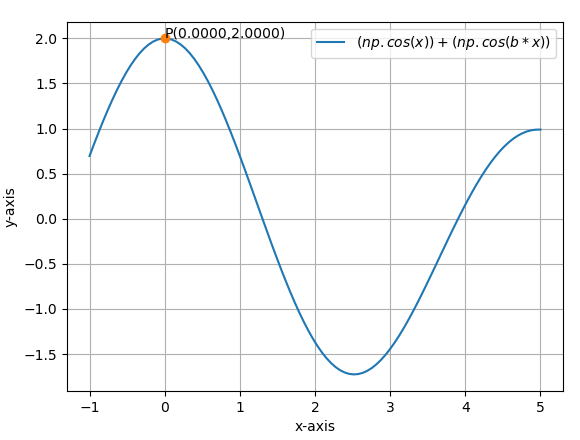
\includegraphics[scale=0.3]{op.png} \\
\end{center} 
%---------------Solution--------------------%
\section*{\large Solution}
 Given function is,
 \begin{align}
	\label{eq:vol_varx}
	f(x) = cosx+cos\sqrt{2}x\\
	\end{align}
	\textbf{Objective function:}
	\begin{align}
	f(x)=\max_x cosx+cos\sqrt{2}x\\
        \end{align}
	\textbf{constraints:}\\
	\begin{align}
		x \in \mathbb{R}
	\end{align}
	\subsection*{Calculation using normal differentiation}
\begin{flushleft}
Differentiating (1) yields,
\end{flushleft}
\begin{align}
\nabla f(x) =-\sqrt{2} sin\sqrt{2}x-sinx
\end{align}
\begin{flushleft}
\subsection*{Calculation of Maxima using gradient ascent algorithm}
\end{flushleft}
\begin{flushleft}
Maxima of the above equation (1), can be calculated from the following expression,\\
\end{flushleft}

\begin{equation}
        x_{n+1} = x_n + \alpha \nabla f(x_n) 
\end{equation}
\begin{flushleft}
\subsection*{Calculation of Maxima using gradient ascent algorithm}
\end{flushleft}
\begin{align}
f(x) = cosx+cos\sqrt{2}x\\
f'(x) = -\sqrt{2} sin\sqrt{2}x-sinx
\end{align}

\vspace{1mm}
we have to attain the maximum value of x. This can be seen in Figure.Using gradient ascent method we can find its maxima.
\begin{equation}
\implies x_{n+1}=x_n+\alpha(-\sqrt{2} sin\sqrt{2}x-sinx)
\end{equation}

Taking $x_0=0.5,\alpha=0.001$ and precision = 0.00000001, values obtained using python are:
    \begin{align}
        \boxed{\text{Maxima} =1.9999}\\     
        \boxed{\text{Maxima Point} =0.0000,2.0000 }
    \end{align}
    \section*{Theoritical proof}
  Here, f(x) can never be bigger than 2 as it is the sum of two functions who are always less than or equal to 1.
\vspace{0.25cm}\\  
  Then, f(0)=2, hence f(x) has a maximum value of 2. 
  \vspace{0.25cm}\\
  Next note for f(x)=2 we need 
  \begin{align}
  x=2\pi n
  \end{align}
   \begin{align}
   \sqrt{2}x=2\pi m, 
   \end{align}
    
for some n,m $\in$ $\mathbb{Z}$  (n,m are integers).
\vspace{0.25cm}\\
This only has 1 solution at x=0. 
\vspace{0.25cm}\\
 To see this say x$\neq$0. 
 \vspace{0.25cm}\\
 Then n,m$\neq$0.
 \vspace{0.25cm}\\
 Now we substitute the $12^{th}$ equation into the $13^{th}$ to get
 \begin{align}
 \sqrt{2}(2\pi n)=2\pi m
\end{align} 
 so,
 \begin{align}
 \sqrt{2} n= m
\end{align} 
Since n,m$\neq$0 this would imply $
\sqrt{2}$ is rational which is clearly a contradiction.
\vspace{0.25cm}\\
Hence, after attaining maximum value at x=0 ,i.e. f(0)=2
f(x) will not attain any maximum value.
 \section*{Conclusion}
\begin{flushleft}
1. At first, the given function has been differentiated and it is solved by setting f'(x) equal to zero. By using x values, f(x) values are calculated.\\
\vspace{0.25cm}
2. Later, the given function f(x) is solved by gradient ascent algorithm to find maxima and the point at which f(x) is maximum.\\
\vspace{0.25cm}
3. Then, the given function f(x) is solved by gradient descent algorithm to find minima and the point at which f(x) is is minimum.\\
\vspace{0.25cm}
\end{flushleft} 
 From this we can say that there is 1 maximum point for the function f(x)
\raggedright  Download the code 
\vspace{0.25cm}\\
\boxed{Github link: \href{https://github.com/RupaSaiSreshta/FWC}{https://github.com/RupaSaiSreshta/FWC}}
\vspace{0.2cm}\\ 

    
  \end{multicols}
\end{document}
